%%%%%%%%%%%%%%%%%%%%%%%%%%%%%%%%%%%%%%%%%%%%%%%%%%%%%%%%%%%%%%%%%%%%%%
% Overleaf (WriteLaTeX) Example: Molecular Chemistry Presentation
%
% Source: http://www.overleaf.com
%
% In these slides we show how Overleaf can be used with standard 
% chemistry packages to easily create professional presentations.
% 
% Feel free to distribute this example, but please keep the referral
% to overleaf.com
% 
%%%%%%%%%%%%%%%%%%%%%%%%%%%%%%%%%%%%%%%%%%%%%%%%%%%%%%%%%%%%%%%%%%%%%%

\documentclass{beamer}

\mode<presentation>
{
  \usetheme{Madrid}       % or try default, Darmstadt, Warsaw, ...
  \usecolortheme{default} % or try albatross, beaver, crane, ...
  \usefonttheme{default}    % or try default, structurebold, ...
  \setbeamertemplate{navigation symbols}{}
  \setbeamertemplate{caption}[numbered]
} 

\usepackage[english]{babel}
\usepackage[utf8x]{inputenc}
\usepackage{chemfig}
\usepackage[version=3]{mhchem}

\usepackage{hyperref}
  \hypersetup{colorlinks=true}
  \hypersetup{urlcolor=blue}
  \hypersetup{linkcolor = .}
\usepackage{xcolor}
\usepackage{siunitx}
  \sisetup{separate-uncertainty = true}
\usepackage{physics}
\usepackage[font=small,labelfont=bf]{caption}
\usepackage{subcaption}
\usepackage[en-GB]{datetime2}
\usepackage{feynmp}
\DeclareGraphicsRule{*}{mps}{*}{}

% Here's where the presentation starts, with the info for the title slide
\title[Graduate Symposium]{Anomalous Cherenkov rings in the DELPHI detector:\\A search for tachyons}
\author{Martin Tat}
\institute{University of Oxford}
\date{15th February 2021}

\titlegraphic{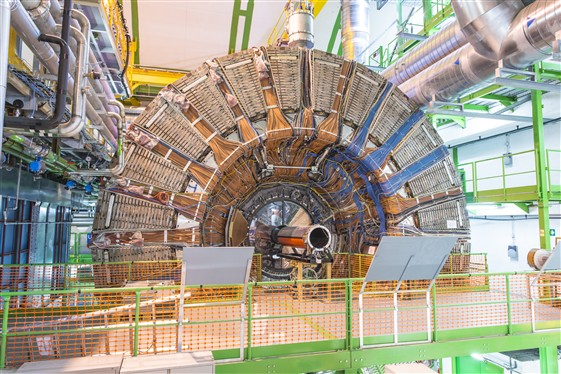
\includegraphics[width = 5cm, height = 3cm]{DELPHI_CERN.jpg}\hspace{1cm}~%
              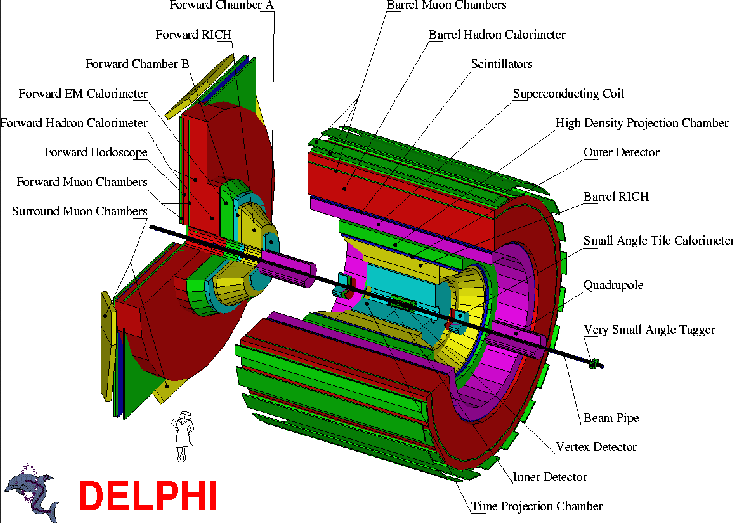
\includegraphics[width = 5cm, height = 3cm]{delphi.png}}

\begin{document}

\begin{frame}
  \titlepage
\end{frame}

% These three lines create an automatically generated table of contents.
\begin{frame}{Outline}
  \tableofcontents
\end{frame}

\section{Introduction}
\begin{frame}{Introduction}
  \begin{itemize}
    \item{Introduce DELHPI and RICH, the authors, paper link}
  \end{itemize}
\end{frame}

\section{Tachyon particles}
\begin{frame}{Tachyon particles}
  \begin{itemize}
    \item{Introduce theory of tachyons}
  \end{itemize}
\end{frame}

\section{DELPHI RICH}
\begin{frame}{DELPHI RICH}
  \begin{itemize}
    \item{Demonstrate how RICH at DELPHI worked and how rings can be anomalous}
  \end{itemize}
\end{frame}

\section{Event topologies and candidate selection}
\begin{frame}{Event topologies and candidate selection}
  \begin{itemize}
    \item{Go through each topology, explain their signatures and show plots of these signatures}
  \end{itemize}
\end{frame}

\section{Analysis results}
\subsection{Correlation between RICH detectors}
\begin{frame}{Correlation between RICH detectors}
  \begin{itemize}
    \item{Show results of the correlation between the two RICH}
  \end{itemize}
\end{frame}

\subsection{Tachyon mass parameters}
\begin{frame}{$K_S^0$ veto}
  \begin{itemize}
    \item{Show the calculated mass parameters}
  \end{itemize}
\end{frame}

\subsection{Kinematic fit}
\begin{frame}{$K_S^0$ veto}
  \begin{itemize}
    \item{Explain the kinematic fitting and show the results}
  \end{itemize}
\end{frame}

\section{Conclusion}
\begin{frame}{Conclusion}
  \begin{itemize}
    \item{Conclude and mention the prospects of tachyon physics at ALICE}
  \end{itemize}
\end{frame}

\end{document}